\begin{figure}[h!tb]
    \centering
    \captionsetup{type=plot}
    \caption{\label{plot:array}Run times by array size}
    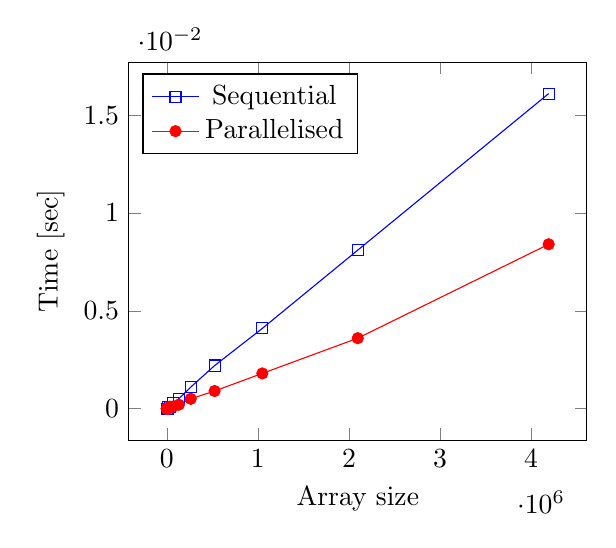
\begin{tikzpicture}
        \begin{axis}[
            title={},
            xlabel={Array size},
            ylabel={Time [sec]},
            legend pos=north west,
            grid style=dashed,
            width=7.4cm,
        ]
            \addplot[
                color=blue,
                mark=square,
                ]
                coordinates {
                    (16,0)
                    (32,0)
                    (64,0)
                    (128,0)
                    (256,0)
                    (512,0)
                    (1024,0)
                    (2048,0)
                    (4096,0)
                    (8192,0)
                    (16384,0.0001)
                    (32768,0.0001)
                    (65536,0.0003)
                    (131072,0.0005)
                    (262144,0.0011)
                    (524288,0.0022)
                    (1048576,0.0041)
                    (2097152,0.0081)
                    (4194304,0.0161)
                };
            
            \addplot[
                color=red,
                mark=*,
                ]
                coordinates {
                    (16,0)
                    (32,0)
                    (64,0)
                    (128,0)
                    (256,0)
                    (512,0)
                    (1024,0)
                    (2048,0)
                    (4096,0)
                    (8192,0)
                    (16384,0)
                    (32768,0.0001)
                    (65536,0.0001)
                    (131072,0.0002)
                    (262144,0.0005)
                    (524288,0.0009)
                    (1048576,0.0018)
                    (2097152,0.0036)
                    (4194304,0.0084)
                };
            \legend{Sequential, Parallelised}
        \end{axis}
    \end{tikzpicture}
\end{figure}